\documentclass[12pt]{article}
\usepackage[margin=1in]{geometry}
\usepackage{amsmath}
\usepackage{amssymb}
\usepackage{graphicx}
\usepackage{booktabs}
\usepackage{hyperref}
\usepackage{xcolor}
\usepackage{makecell}
\usepackage{float}

\title{Continued Fractions for Constants and Functions}
\author{Carter Mitchell, Sydney Spacek}
\date{\today}

\begin{document}
\maketitle

\subsection*{AI Disclosure}
No AI tools were used.

\subsection*{Author Contributions}
\noindent
\textbf{Who Coded What:} \\
Carter Mitchell: 55\verb|%| (Lead)
\begin{itemize}
    \item Project 2 parts 1 through 3.
    \item Code implementation of a backward recurrence continued fraction method.
    \item Implemented five constants and five functions.
    \item Led the GitHub repository and general file updates.
\end{itemize}

\noindent
Sydney Spacek: 45\verb|%|
\begin{itemize}
    \item Project 2 parts 4 through 6.
    \item Code implementation of a forward recurrence continued fraction method.
    \item Implemented figures and tables of data.
    \item Supported the GitHub repository with batch updates.
\end{itemize}

\noindent
\textbf{Who Wrote What:} \\
Carter Mitchell: 45\verb|%|
\begin{itemize}
    \item Wrote the methods, references, and appendix sections.
    \item Compiled the constant and function rules in the appendix table.
    \item Wrote the README.
\end{itemize}

\noindent
Sydney Spacek: 55\verb|%| (Lead)
\begin{itemize}
    \item Background and results sections.
    \item Compiled the figures and tables of data.
\end{itemize}

\subsection*{Background}
There are many examples of continued fractions being used throughout history. Some famous instances of continued fractions are Euler's infinite series, Brouncker’s formula, and Johann Heinrich Lambert's proof of the irrationality of pi.

A continued fraction is a nested fraction. This means that when written the denominator of the fraction is itself a fraction, whose denominator is a fraction, and so on. When a continued fraction is written it has the form:
\begin{equation}
    b_0+\dfrac{a_1}{b_1+\dfrac{a_2}{b_2+\dfrac{a_3}{b_3+\dots}}}
    \label{fraction}
\end{equation}

Continued fractions can be solved multiple ways. One way is through backward recurrence, where you solve from the bottom of the fraction on up. Another way is through forward recurrence, where you solve from the top on down.

\subsection*{Methods}

We used the continued fraction formula \eqref{fraction} to combine results from various sources of constants and functions expressed in a continued fraction form. Across both backward and forward recurrence methods we computed up to a depth of $N$. For the backward recurrence method, we initialized the continued fraction function with the lowest fraction 
\begin{align*}
    F_N = \dfrac{a_N}{b_N},
\end{align*}
and built up to the top and total fraction $F_0 = b_0+F_1$, where each fraction was built with the recurrence relation
\begin{equation*}
    F_i = \dfrac{a_{i}}{b_{i}+F_{i+1}} \text{ for } i\in\{1,...,N-1\}.
\end{equation*}
For the forward recurrence method, we initialized the continued fraction function with
\begin{align*}
    A_{-1} &=1, \\
    A_0 &=b_0, \\
    B_{-1} &= 0, \\
    B_0 &= 1,
\end{align*}
followed by computing all the partial numerators $A_i$ and denominators $B_i$ for $i\in\{1,...,N\}$, where partial fractions $\dfrac{A_i}{B_i}$ were built with the recurrence relations
\begin{align*}
    A_i &= b_iA_{i-1}+a_iA_{i-2}, \\
    B_i &= b_iB_{i-1}+a_iA_{i-2}.
\end{align*}

All constants, functions, and rules for $a_i$ and $b_i$ including their respective references can be found in Table \ref{tab:generalized_fraction_table} of Appendix A.

\subsection*{Results}
The results from the constants are represented through two types of error. The results of these error calculations are shown in Table \ref{tab:values} and Figures 1 through 6 below.
\begin{table}[H]
  \centering
  \begin{tabular}{c c c c}
    \toprule
    Constants & Equations & Absolute Error & Relative Error \\
    \midrule
    First & $\pi/4$ & 0.000025 & 0.000032 \\
    Second & $e$ & 0.0 & 0.0 \\
    Third & $30/(\pi^2)$ & 0.0 & 0.0 \\
    Fourth & $1/(2G)$ & $6.2792246445855792736(10^{-17})$ & $1.1503107465100134020(10^{-16})$ \\
    Fifth & $1/(1-\log(2))$ & 0.0 & 0.0 \\
    \bottomrule
  \end{tabular}
  \caption{The Constant Calculation Error with $N=10000$}
  \label{tab:values}
\end{table}
The first constant plot on the left of Figure \ref{fig:one} shows the error of the first constant as $N$ increases at points 50, 100, 500, 1000, 5000, 10000. The second constant plot on the right shows the error of the second constant as $N$ increases at points 5, 10, 50, 100, 500, 1000.
\begin{figure}[H]
  \centering
  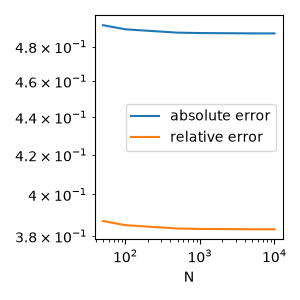
\includegraphics[width=0.35\textwidth]{plot1.png}
  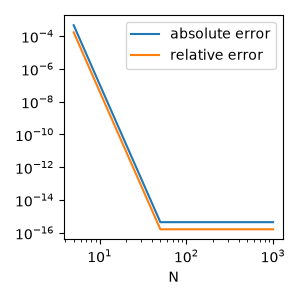
\includegraphics[width=0.35\textwidth]{plot2.png}
  \caption{left plot presents first constant error and right plot presents second constant error}
  \label{fig:one}
\end{figure}

The third constant plot on the left of Figure \ref{fig:two} shows the error of the third constant as $N$ increases at points 1, 2, 3, 4, 5, 6. The fourth constant plot on the right shows the error of the fourth constant as $N$ increases at points 50, 100, 500, 1000, 5000, 10000.
\begin{figure}[H]
  \centering
  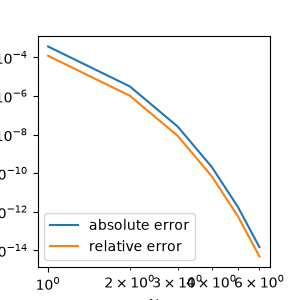
\includegraphics[width=0.35\textwidth]{plot3.png}
  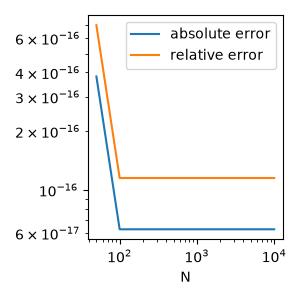
\includegraphics[width=0.35\textwidth]{plot4.png}
  \caption{left plot presents third constant error and right plot presents fourth constant error}
  \label{fig:two}
\end{figure} 
The fifth constant plot in Figure \ref{fig:three} shows the error of the fifth constant as $N$ increases at points 1, 2, 3, 4, 5, 10, 15, 20.
\begin{figure}[H]
  \centering
  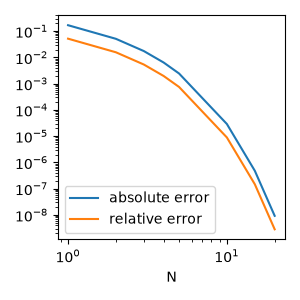
\includegraphics[width=0.35\textwidth]{plot5.png}
  \caption{the plot presents fifth constant error}
  \label{fig:three}
\end{figure}
The results from the function section are represented by the error plotted against the results of the actual functions. the results were calculated using $x=7$ and $N=10000$. The figures are as follows.
\begin{figure}[H]
  \centering
  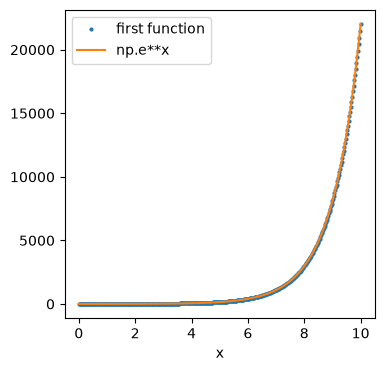
\includegraphics[width=0.35\textwidth]{equation 1.png}
  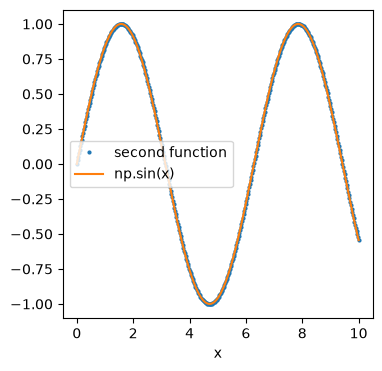
\includegraphics[width=0.35\textwidth]{equation 2.png}
  \caption{left plot presents the first function and right plot presents the second function}
  \label{fig:four}
\end{figure}

\begin{figure}[H]
  \centering
  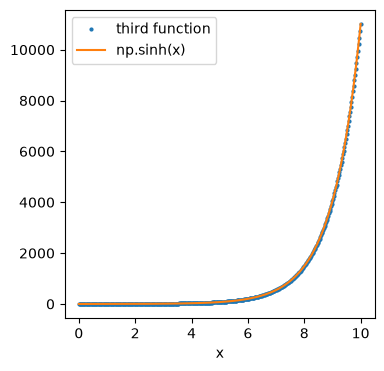
\includegraphics[width=0.35\textwidth]{equation 3.png}
  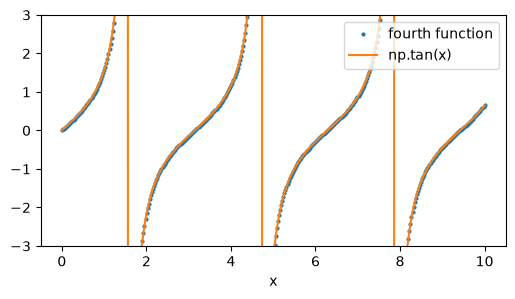
\includegraphics[width=0.35\textwidth]{equation 4.png}
  \caption{left plot presents the third function and right plot presents the fourth function}
  \label{fig:five}
\end{figure}

\begin{figure}[H]
  \centering
  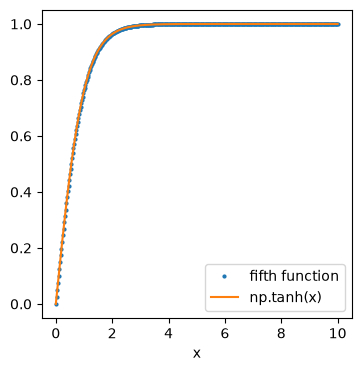
\includegraphics[width=0.35\textwidth]{equation 5.png}
  \caption{Fifth Function}
  \label{fig:six}
\end{figure}

\newpage
\bibliographystyle{unsrt}
\bibliography{ReportBibliography}

\newpage
\begin{center}
    \subsection*{Appendix A}{\large}
\end{center}

All constants, functions, and rules for $a_i$ and $b_i$ including their respective source references can be found in Table \ref{tab:generalized_fraction_table}.

% Add vertical space to each row
\setcellgapes{3pt}
\makegapedcells

\begin{table}[h!]
\centering
% resize box used inside table object to center the tabular object
\resizebox{\textwidth}{!}{%
    \begin{tabular}{c|c|c}
    
    Constant or Function & $a_i$ & $b_i$ \\

    % First Constant
    \hline
    $\dfrac{\pi}{4}$ \cite{first_constant:wikipedia} & $(2i-3)^2$ & $\begin{cases}
        0, i=0 \\
        1, i = 1 \\
        2, i\notin\{0,1\}
    \end{cases}$ \\

    % Second Constant
    \hline
    $e$ \cite{second_constant:blog} & $1$ & $\begin{cases}
        2, i=0 \\
        \tfrac{2i+1}{3}, i\equiv2\pmod{3} \\
        1, \text{otherwise}
    \end{cases}$ \\

    % Third Constant
    \hline
    $\dfrac{30}{\pi^{2}}$ \cite{third_constant:ramanujanmachine} & $i^4$ & $11i^2+11i+3$ \\

    % Fourth Constant
    \hline
    $\dfrac{1}{2G}$ for Catalan's constant $G$ \cite{fourth_constant:ramanujanmachine} & $-2i^4$ & $3i^2+3i+1$ \\

    % Fifth Constant
    \hline
    $\dfrac{1}{1-\ln{2}}$ \cite{fifth_constant:ramanujanmachine} & $-2i^2(i+1)^2$ & $3i^2+7i+4$ \\

    % First Function
    \hline
    $e^{x}$ \cite{first_function:wikipedia} & $\begin{cases}
        1,i=1 \\
        \tfrac{-x}{i-1},i\ne1
    \end{cases}$ & $\begin{cases}
        0,i=0 \\
        1,i=1 \\
        1+\tfrac{x}{i-1},i\notin\{0,1\}
    \end{cases}$ \\

    % Second Function
    \hline
    $\sin{x}$ \cite{second_function:wikipedia} & $\begin{cases}
        x,i=1 \\
        x^2,i=2 \\
        (2i-4)(2i-3)x^2,i\notin\{1,2\}
    \end{cases}$ & $\begin{cases}
        0,i=0 \\
        1,i=1 \\
        (2i-2)(2i-1)-x^2,i\notin\{0,1\}
    \end{cases}$ \\

    % Third Function
    \hline
    $\sinh{x}$ \cite{third_function:wikipedia} & $\begin{cases}
        x,i=1 \\
        -x^2,i=2 \\
        (4-2i)(2i-3)x^2, i\notin\{1,2\}
    \end{cases}$ & $\begin{cases}
        0,i=0 \\
        1,i=1 \\
        (2i-2)(2i-1)+x^2,i\notin\{0,1\}
    \end{cases}$ \\

    % Fourth Function
    \hline
    $\tan{x}$ \cite{fourth_function:blog} & $\begin{cases}
        x,i=1 \\
        -x^2,i\ne1
    \end{cases}$ & $\begin{cases}
        0,i=0 \\
        2i-1,i\ne0
    \end{cases}$ \\

    % Fifth Function
    \hline
    $\tanh{x}$ \cite{fifth_function:wikipedia} & $1$ & $\begin{cases}
        0,i=0 \\
        \tfrac{2i-1}{x},i\ne0
    \end{cases}$
    
    \end{tabular}%
    }
    \caption{Generalized Fraction Rules for Constants and Functions}
    \label{tab:generalized_fraction_table}
\end{table}

\end{document}
